% Customer Fit Intelligence: the paper, in an IEEE conference layout (T808;
% revised after two outside reviews in T810).
% The layout is set by hand to match IEEEtran, so any TeX Live builds it:
% US letter, two 3.5 in columns 0.25 in apart, 10 pt Times. Build with
% pdflatex three times; SOURCES.md says where every number comes from, and
% SUPPLEMENT.md gives every setting and the tables the page limit leaves out.
\documentclass[10pt,twocolumn,letterpaper]{article}

\usepackage[letterpaper,top=0.75in,bottom=1in,left=0.625in,right=0.625in,columnsep=0.25in]{geometry}
\usepackage[T1]{fontenc}
\usepackage{mathptmx}
\renewcommand{\ttdefault}{lmtt} % a vector typewriter font for URLs (no bitmap fonts)
\usepackage{amsmath,amssymb}
\usepackage{graphicx}
\usepackage{booktabs}
\usepackage{array}
\usepackage{xcolor}
\usepackage{tikz}
\usetikzlibrary{arrows.meta,positioning}
\usepackage{titlesec}
\usepackage[font=footnotesize,labelsep=period,skip=4pt]{caption}
\usepackage{enumitem}
\usepackage{microtype}
\usepackage{cite}
\usepackage{flushend}
\usepackage[hidelinks]{hyperref}
\usepackage{url}

% IEEE headings: I. INTRODUCTION (small caps, centred); A. Setup (italic)
\renewcommand{\thesection}{\Roman{section}}
\renewcommand{\thesubsection}{\thesection-\Alph{subsection}}
\titleformat{\section}{\centering\normalsize\scshape}{\Roman{section}.}{0.5em}{}
\titlespacing*{\section}{0pt}{9pt}{4pt}
\titleformat{\subsection}{\normalsize\itshape}{\Alph{subsection}.}{0.5em}{}
\titlespacing*{\subsection}{0pt}{6pt}{2pt}
\setlength{\parindent}{1em}
\setlength{\parskip}{0pt}

% IEEE captions: TABLE I above, small caps; Fig. 1. below
\DeclareCaptionLabelFormat{ieeetable}{\textsc{Table}~#2}
\captionsetup[table]{labelformat=ieeetable,labelsep=newline,justification=centering,textfont=sc}
\captionsetup[figure]{name=Fig.,justification=justified,singlelinecheck=false}
\renewcommand{\thetable}{\Roman{table}}
% A section reference that never breaks across a line: Section~V-D
\newcommand{\secref}[1]{Section~\mbox{\ref{#1}}}

\newcommand{\runin}[1]{\textit{#1}\hspace{0.4em}}
\setlist{leftmargin=1.4em,itemsep=1pt,topsep=2pt}
\raggedbottom
\hyphenation{Respect Lovemark Lovemarks}

\begin{document}

\twocolumn[{%
\begin{center}
{\fontsize{22}{26}\selectfont Customer Fit Intelligence: A Theory-Constrained\\[2pt]
Neural Network with Exact Explanations for Customer\\[2pt]
Relationships in Food Delivery\par}
\vspace{12pt}
{\normalsize Charanko\par}
{\small\itshape Web 3 Developer\par}
{\small \href{mailto:aryastark111.as@gmail.com}{aryastark111.as@gmail.com}\par}
\vspace{14pt}
\end{center}
}]

\noindent\textbf{\textit{Abstract}---Churn models tell a delivery business who may leave, but rarely why. Customer Fit Intelligence (CFI) is a neural network whose structure comes from marketing theory: each order becomes eight expectation gaps, which feed Respect and Love, the axes of Roberts' love matrix, then Trust and Convenience, then one Fit score that drives reorders, churn and the Net Promoter Score answer. Fifteen allowed paths, positive weights and a steeper response to shortfalls leave 21 parameters between an order and its Fit, and with eight inputs every score's Shapley values are computed exactly. We study it in 20 simulated populations whose hidden model shares CFI's structure, so the study checks cost and identifiability when the theory is right. There CFI's churn AUC (0.802) is within 0.003 of the best of five comparators on the same inputs, its states follow the hidden ones (correlation 0.975 to 0.988, against 0.75 to 0.93 for untrained equal weights), and with purchase history it comes within 0.003 of a model that knows the true Fit. With only what today's events measure, flexible models do better. Survey anchors keep CFI accurate with 100 training customers, and its driver ranking finds planted problems at restaurants and couriers from about 200 customers. On 95,824 real e-commerce orders, lateness costs more than earliness earns, by a factor between 3 and 12 depending on the reviews and range used, while fees show the reverse. CFI runs as a cloud service with a dashboard, and we report its latency and cost.}

\vspace{6pt}
\noindent\textbf{\textit{Index Terms}---churn prediction, interpretable machine learning, theory-guided neural networks, Shapley values, customer relationship management, food delivery.}

\section{Introduction}

A food-delivery customer who stops ordering rarely says why. Churn models can say who is likely to leave, often well, but are judged on who and seldom asked why \cite{neslin2006}; models built on purchase history alone, such as BG/NBD \cite{fader2005}, forecast repeat purchases with no view of the service a customer received. A business that wants to keep customers needs both: an early and accurate risk, and the reason behind it, for one order, one restaurant or one courier.

Customer Fit Intelligence (CFI) is a small neural network whose structure comes from marketing theory and whose strengths come from data. It turns each order into eight expectation gaps, how much better or worse than expected the speed, ease, fees, accuracy, courier, food, personalisation and support were \cite{oliver1980}, and lets theory fix how those gaps may combine: which states each may move, in which direction, and with shortfalls weighing more than equal surpluses \cite{mittal1998}. The states are the axes of Roberts' love matrix, Respect and Love \cite{roberts2004}, and from them Trust, Convenience and finally Fit, which drives reorders, churn and the answer behind the Net Promoter Score \cite{reichheld2003}.

Constraining a network this way raises two questions: does it cost accuracy against models free to learn any function of the same inputs, and does training recover the states it names? No real data comes with known states, so we study both on a simulator whose hidden model shares CFI's connections and signs \cite{morris2019}: a check under correct specification, which shows what the constraints cost when the theory is right, not that real customers have these states. We then break the theory one assumption at a time, test the gap and asymmetry ideas on 95,824 public e-commerce orders \cite{olist2018}, and run the system as a service. Our contributions are four:
\begin{enumerate}
\item CFI, a theory-constrained network with 15 allowed paths and 21 parameters from gaps to Fit, whose hidden units are named states with fixed directions, each score explained by exact Shapley values over 256 coalitions \cite{lundberg2017,sundararajan2020}.
\item A simulation study in 20 populations with paired comparisons: CFI predicts within 0.004 AUC of the best comparator, its states follow the truth beyond what the structure alone gives, anchors let it learn from 100 customers, and its drivers find planted problems once groups have enough orders.
\item A test on real orders: lateness costs more than earliness earns, by an amount that depends on when reviews were written, and fees run the other way.
\item A running system, from events through transactional scoring and a model registry to a dashboard, with latency and cost measured.
\end{enumerate}
\secref{sec:theory} sets out the theory, \secref{sec:data} the data, \secref{sec:model} the model, \secref{sec:experiments} the experiments and \secref{sec:system} the system; \secref{sec:discussion} discusses limitations and \secref{sec:conclusion} concludes.

\section{Theory and Related Work}\label{sec:theory}

Four ideas set CFI's structure.

\runin{Gaps against expectations.} Satisfaction depends on the gap between what happened and what the customer expected \cite{oliver1980}, not only on the level of performance. Every CFI input is such a gap, signed so that positive always means better than expected: delivery minutes against the promised time, and every other measure against the customer's own running baseline (\secref{sec:data}).

\runin{Asymmetry.} A shortfall lowers satisfaction and repurchase more than an equal surplus raises them \cite{mittal1998}. Each gap $d$ is therefore multiplied by a learned $\kappa > 1$ when it is negative (\secref{sec:model}).

\runin{Relational states.} Roberts places a brand on two axes: Respect, earned by performance, and Love, earned by emotional connection \cite{roberts2004}. High on both is a Lovemark; high on Respect alone a Brand; high on Love alone a Fad; low on both a Product. CFI scores every customer on the same two axes. Trust, central to relationship marketing \cite{morgan1994}, grows from both, and Convenience from the time and effort a service saves \cite{berry2002}. Together they form Fit: how well the service suits this customer. Fit drives three observable outcomes: reordering, churn and the 0-to-10 likelihood-to-recommend answer behind the Net Promoter Score (the NPS answer) \cite{reichheld2003}. Theory motivates these paths but does not settle all of them: it does not say exactly which attributes earn Respect rather than Love, that food feeds both, or that fees, a cost rather than an effort, feed Convenience. We treat the 15 paths as a design hypothesis, which \secref{sec:recovery} tests by removing each one and \secref{sec:robust} by adding two.

\runin{Models that explain.} Churn models are usually judged by lift and AUC alone \cite{neslin2006}, and buy-till-you-die models such as BG/NBD forecast repeat purchases from frequency and recency without saying why a customer drifts \cite{fader2005}. Gradient boosting \cite{friedman2001} and unconstrained networks predict well and can be explained after the fact, input by input, with Shapley values \cite{lundberg2017}, but their intermediate computations carry no meaning and an input's effect may change sign. Rudin argues for models interpretable by construction \cite{rudin2019}, and theory-guided data science fixes a model's structure from domain knowledge while learning its strengths from data \cite{karpatne2017}. Concept bottleneck models predict through named, supervised intermediate concepts \cite{koh2020}; CFI's states play that role, supervised by survey items and behaviours. Monotonic networks guarantee the direction of each input's effect \cite{you2017}; CFI gets that from positive weights on a sparse mask. Satisfaction-index models such as the ACSI fix paths between latent constructs from theory and estimate them by structural equations \cite{fornell1996}; CFI learns such paths per order, from behavioural data, in a network that serves predictions.

\section{Data}\label{sec:data}

CFI learns from the events an ordering app already sends, turned into eight gaps per order, two outcome labels and sparse survey answers.

\runin{Events.} Event schema v1 defines eleven event types: nine describe the customer journey (an order placed, delivered or gone wrong, a rating, an app session, a recommendation shown or clicked, a support case, a survey answer) and two record automated actions. Every event is checked against its schema on arrival; one that fails is refused, never stored.

\runin{From events to gaps.} Table~\ref{tab:inputs} shows how each input is measured. Speed is judged against the promised time; every other measure against the customer's own expectation, an exponentially weighted mean (weight 0.3 once warmed up) blended with a population prior $\mu_0$, a fixed constant per input. A new customer starts from the prior (blend weight $w/(w+3)$ after $w$ orders), and a lapsed one drifts back to it as $w$ halves every 60 days without an order. Formally, for a measure $y$ with running mean $m$, weight $w$ (in orders) and $\Delta t$ days since the customer was last seen, the weight first decays and the gap is taken against the blended expectation:
\begin{equation}
w \leftarrow w\,2^{-\Delta t/60}, \quad \hat{y} = \frac{w\,m + 3\,\mu_0}{w + 3}, \quad d = \pm\,(y - \hat{y}),
\end{equation}
with the sign chosen so that positive is better; then the order updates the habit:
\begin{equation}
a = \max\!\left(0.3, \tfrac{1}{w+1}\right), \quad m \leftarrow a\,y + (1-a)\,m, \quad w \leftarrow w + 1.
\end{equation}
An input an order did not measure counts as 0, ``as expected''.

\begin{table}[t]
\caption{The Eight Inputs}\label{tab:inputs}
\centering\footnotesize
\setlength{\tabcolsep}{4pt}
\begin{tabular}{@{}l l p{4.1cm}@{}}
\toprule
Input & Name & Measured from \\
\midrule
$x_1$ & Speed vs promise & promised minus actual delivery minutes \\
$x_2$ & App ease & seconds from app open to checkout \\
$x_3$ & Fee load & fees divided by basket value \\
$x_4$ & Order fidelity & share of items right (v1 events carry no item counts) \\
$x_5$ & Courier conduct & courier rating, 1 to 5 \\
$x_6$ & Food \& selection & food rating, 1 to 5 \\
$x_7$ & Personalisation & share of recommendations shown that were clicked (no v1 rule pairs them yet) \\
$x_8$ & Recovery handling & support-case satisfaction, 1 to 5 \\
\bottomrule
\end{tabular}
\par\smallskip\parbox{\columnwidth}{\footnotesize $x_1$ is a gap against the promise, positive when early; $x_2$ to $x_8$ are gaps against the customer's own baseline, with the sign of $x_2$ and $x_3$ flipped so that positive means faster or cheaper.}
\end{table}

\runin{Outcomes and anchors.} Each order gets two labels from the order history that follows it: reorder within 14 days, and churn when 30 days pass with no new order. A label stays unknown while its window is open, unless a later order already settles it; so the last days of data hold reorders and no churn, and \secref{sec:prediction} checks that this changes no comparison. After some orders the app asks one rotating question: the NPS question (0 to 10) or a 1-to-7 item for Respect, Love, Trust or Convenience. Those four states also have one or two behaviours each: favourites saved and the share of orders without a promotion for Love, the average rating for Respect, trying new restaurants and saving a payment method for Trust, and time to checkout for Convenience. Fit has no item or behaviour; the outcomes anchor it.

\runin{Simulated populations.} Real customer data are not yet available, so the study uses a simulator with known ground truth \cite{morris2019}. Its hidden model has the same connections and signs as CFI, a separate $\kappa$ per input (1.2 to 3.0, mean 1.96) and Fit $= \sigma(5\,\text{Trust} + 3\,\text{Convenience} - 4.3)$; outcomes follow the true Fit, and survey answers and behaviours follow the true states. Each population has 2,000 customers ordering every 7 days or so over 180 days, from 40 restaurants and 60 couriers; about one order in ten goes wrong, 30\% of orders are rated, and every order that went wrong is rated. Twenty populations (seeds 2026 to 2045) are each split 80/20 by customer; in the first, 1,600 customers (35,707 orders) train the model and 400 (8,520 orders) are held out. For the driver tests, the simulator can plant problems: 80\% of one kind of incident moved to a few named restaurants or couriers, so only where incidents happen changes, not how many. The supplement gives every setting, and the code is public (\secref{sec:discussion}).

\section{Model}\label{sec:model}

CFI is a three-layer neural network whose 15 connections are fixed by theory and whose strengths are learned: 21 parameters (15 weights, 5 biases and $\kappa$) carry an order's gaps to Fit, and 52 in all, with 15 in the outcome heads and 16 in the anchors.

\begin{figure}[t]
\centering
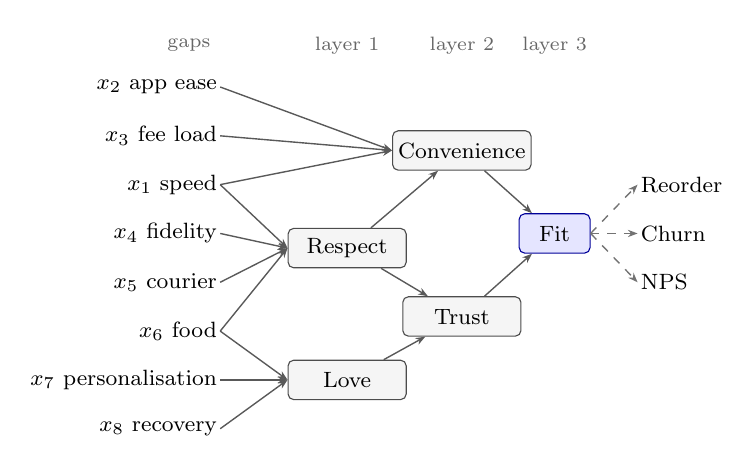
\begin{tikzpicture}[x=0.62cm, y=0.62cm,
  >={Stealth[length=3.5pt]}, font=\footnotesize,
  inp/.style={anchor=east, inner sep=1pt},
  st/.style={draw=black!70, rounded corners=2pt, fill=black!4, minimum width=1.5cm, minimum height=0.5cm, inner sep=2pt},
  fit/.style={st, fill=blue!10, draw=blue!60!black, minimum width=0.9cm},
  head/.style={anchor=west, inner sep=1pt},
  link/.style={->, draw=black!65, line width=0.5pt},
  headarrow/.style={->, draw=black!55, dashed, line width=0.5pt}]
\node[inp] (x2) at (0, 3.5) {$x_2$ app ease};
\node[inp] (x3) at (0, 2.5) {$x_3$ fee load};
\node[inp] (x1) at (0, 1.5) {$x_1$ speed};
\node[inp] (x4) at (0, 0.5) {$x_4$ fidelity};
\node[inp] (x5) at (0,-0.5) {$x_5$ courier};
\node[inp] (x6) at (0,-1.5) {$x_6$ food};
\node[inp] (x7) at (0,-2.5) {$x_7$ personalisation};
\node[inp] (x8) at (0,-3.5) {$x_8$ recovery};
\node[st] (R) at (2.6, 0.2) {Respect};
\node[st] (L) at (2.6,-2.5) {Love};
\node[st] (C) at (4.95, 2.2) {Convenience};
\node[st] (T) at (4.95,-1.2) {Trust};
\node[fit] (F) at (6.85, 0.5) {Fit};
\foreach \s in {x1,x4,x5,x6} \draw[link] (\s.east) -- (R.west);
\foreach \s in {x6,x7,x8} \draw[link] (\s.east) -- (L.west);
\foreach \s in {x1,x2,x3} \draw[link] (\s.east) -- (C.west);
\draw[link] (R) -- (C);
\draw[link] (R) -- (T);
\draw[link] (L) -- (T);
\draw[link] (C) -- (F);
\draw[link] (T) -- (F);
\node[head] (h1) at (8.55, 1.5) {Reorder};
\node[head] (h2) at (8.55, 0.5) {Churn};
\node[head] (h3) at (8.55,-0.5) {NPS};
\foreach \h in {h1,h2,h3} \draw[headarrow] (F.east) -- (\h.west);
\node[font=\scriptsize, text=black!60] at (0.0, 4.35) [anchor=east] {gaps};
\node[font=\scriptsize, text=black!60] at (2.6, 4.35) {layer 1};
\node[font=\scriptsize, text=black!60] at (4.95, 4.35) {layer 2};
\node[font=\scriptsize, text=black!60] at (6.85, 4.35) {layer 3};
\end{tikzpicture}
\caption{The CFI network. Solid arrows are the 15 paths the theory allows; dashed arrows are the outcome heads (reorder within 14 days, churn within 30 days, the NPS answer). Respect, Love, Convenience and Trust are each also anchored by a survey item and one or two behaviours (not drawn); Fit only by the outcomes.}\label{fig:network}
\end{figure}

\runin{Structure.} Input $x_i$'s gap $d_i$ passes through the asymmetric transform, with one $\kappa$ shared by all eight inputs, and is divided by a fixed scale $s_i$, the root mean square of $d_i$ over the training orders:
\begin{equation}
z_i = \frac{g_\kappa(d_i)}{s_i}, \qquad g_\kappa(d) = \begin{cases} d, & d \geq 0, \\ \kappa d, & d < 0, \end{cases}
\end{equation}
with $\kappa = 1 + \operatorname{softplus}(\theta) > 1$. Each layer $l$ is a sigmoid of a masked linear map of its input $u^{(l)}$ with non-negative weights:
\begin{equation}
h^{(l)} = \sigma\!\left( \left( \operatorname{softplus}(\Theta^{(l)}) \odot M^{(l)} \right) u^{(l)} + b^{(l)} \right).
\end{equation}
Layer 1 reads $u^{(1)} = z$ and gives Respect and Love; layer 2 reads Respect, Love and $z_1$ to $z_3$ and gives Convenience and Trust; layer 3 reads those two and gives Fit (Fig.~\ref{fig:network}). The masks $M$ hold the theory: Respect reads speed, order fidelity, courier conduct and food ($x_1, x_4, x_5, x_6$); Love reads food, personalisation and recovery ($x_6, x_7, x_8$); Convenience reads Respect, speed, app ease and fees; Trust reads Respect and Love. Of the 28 possible connections, 15 are allowed. A weight off the mask is exactly zero after every optimiser step, and every weight on it is positive, so a better-than-expected gap can never lower a score. States are computed from one order's gaps: a customer's state is that of their latest order, and memory enters only through the expectations behind the gaps.

\runin{Outcome heads.} Fit drives three heads whose slopes have fixed signs: the chance of a reorder within 14 days rises with Fit and the chance of churn within 30 days falls (both logistic), and the NPS answer follows a cumulative-logit model with ten ordered cuts \cite{mccullagh1980}.

\runin{Anchors.} A latent state needs a scale. Each of the four anchored states has a 1-to-7 survey item as its marker: $P(\text{answer} \leq k) = \sigma(\lambda(k/7 - \text{state}))$, with the thresholds fixed at $k/7$ so that a neutral answer sits near 0.5 and only the slope $\lambda > 0$ is learned. Each standardised behaviour follows $c + b \times$ the customer's mean state, with $b > 0$.

\runin{Training.} The loss adds the cross-entropy (CE) of the two binary heads, the ordinal negative log-likelihood (NLL) of the NPS answer and of each of the four items, and the squared error (SE) of each of the six behaviours, every term averaged over the rows where it is observed, plus an L2 penalty on every weight and slope $\beta$:
\begin{multline}
\mathcal{L} = \overline{\mathrm{CE}}_{\mathrm{reorder}} + \overline{\mathrm{CE}}_{\mathrm{churn}} + \overline{\mathrm{NLL}}_{\mathrm{NPS}} \\
+ \sum_{j=1}^{4} \overline{\mathrm{NLL}}_{\mathrm{item}\,j} + \sum_{k=1}^{6} \overline{\mathrm{SE}}_{\mathrm{behaviour}\,k} + 10^{-4} \sum \beta^2.
\end{multline}
Full-batch L-BFGS runs in float64, in rounds of 20 iterations, until the loss changes by at most $10^{-9}$ (relative) between rounds. The learned numbers are exported as model.json, and the API scores with a NumPy copy of the forward pass that matches the PyTorch network to about $10^{-16}$, so serving never needs PyTorch.

\runin{Exact explanations.} For a score $f$ and an order's gaps $d$, input $i$'s contribution is its baseline Shapley value \cite{sundararajan2020}, with an order exactly as expected (every gap 0) as the baseline:
\begin{gather}
\phi_i = \sum_{S \subseteq N \setminus \{i\}} \frac{|S|!\,(7-|S|)!}{8!} \left[ f(d_{S \cup \{i\}}) - f(d_S) \right], \\
\sum_{i=1}^{8} \phi_i = f(d) - f(0).
\end{gather}
Here $N$ is the set of eight inputs, and $d_S$ keeps the gaps in $S$ and sets the others to 0. With eight inputs there are only $2^8 = 256$ coalitions, so CFI computes every contribution exactly, for six scores (the five states and churn risk). Any model of the same inputs could be explained this way; CFI adds that every score is a named state with fixed signs. Contributions are per input, not per path: speed's contribution to Fit is not the sum of its contributions to Respect and Convenience.

\runin{Quadrants.} Respect and Love place each customer in one of Roberts' four quadrants \cite{roberts2004}, split at 0.5 on each axis, where the survey anchors put a neutral answer.

\section{Experiments}\label{sec:experiments}

\subsection{Setup}

The study follows the ADEMP plan for simulation studies \cite{morris2019}. \textit{Aim:} under correct specification, what does fixing the structure cost, and does training recover the named states? \textit{Data:} the 20 simulated populations of \secref{sec:data}, each split 80/20 by customer; recovery and the ablation use the first five, robustness and small data the first three. \textit{Estimands:} each order's chance of churn within 30 days and of a reorder within 14, the five states, and each customer's quadrant. \textit{Methods:} CFI and ten comparators (Table~\ref{tab:prediction}). On the same eight gaps: logistic regression (LR) on the raw gaps, and on each gap's surplus and shortfall as separate columns, so it can weigh shortfalls more as $\kappa$ does; gradient boosting \cite{friedman2001} (scikit-learn, default settings), unconstrained and with CFI's signs as monotonic constraints; and an unconstrained network (two hidden layers of 16, fitted by L-BFGS, its L2 penalty tuned on a fifth of the training customers; it stops at 2,000 iterations, so its AUC varies by up to 0.003 between machines). On purchase history alone: the order rate, and BG/NBD \cite{fader2005}, which gives each held-out order the chance of no order in the next 30 or 14 days. On both: gradient boosting, and CFI's Fit with the same history in a logistic regression. A ceiling uses the simulator's true Fit instead. History uses only earlier orders, so no label leaks into it. \textit{Performance:} AUC, log loss and expected calibration error (ECE, ten bins holding equal numbers of orders) on held-out customers' orders, and CFI's paired difference from each comparator, population by population, with its standard error. We call CFI no worse than a comparator when the 95\% interval of its AUC difference lies above $-0.005$, a margin we set here, not in advance.

\begin{table}[t]
\caption{Held-Out Prediction in 20 Populations}\label{tab:prediction}
\centering\footnotesize
\setlength{\tabcolsep}{3.4pt}
\begin{tabular}{@{}l r r r r@{}}
\toprule
 & \multicolumn{2}{c}{Churn 30 d} & \multicolumn{2}{c}{Reorder 14 d} \\
\cmidrule(lr){2-3}\cmidrule(l){4-5}
Model & AUC & $\Delta$ (SE) & AUC & $\Delta$ (SE) \\
\midrule
\multicolumn{5}{@{}l}{\textit{One order's gaps}} \\
CFI (15 paths) & 0.802 & & 0.729 & \\
LR, raw gaps & 0.798 & 4.4 (1.0) & 0.724 & 4.5 (0.5) \\
LR, surplus/shortfall & 0.804 & $-$2.2 (0.8) & 0.732 & $-$3.4 (0.5) \\
Gradient boosting & 0.784 & 18.1 (1.4) & 0.721 & 7.5 (0.9) \\
Boosting, monotone & 0.798 & 4.4 (1.1) & 0.727 & 1.3 (0.7) \\
Unconstrained network & 0.798 & 3.7 (1.2) & 0.727 & 1.8 (0.8) \\
\multicolumn{5}{@{}l}{\textit{History only}} \\
BG/NBD & 0.664 & 138.4 (4.5) & 0.684 & 44.5 (2.3) \\
Order rate & 0.642 & 159.6 (5.7) & 0.677 & 51.8 (2.6) \\
\multicolumn{5}{@{}l}{\textit{Gaps and history}} \\
CFI Fit + history & 0.817 & & 0.775 & \\
Gradient boosting & 0.798 & 19.2 (1.6) & 0.766 & 9.0 (0.7) \\
True Fit + history & 0.819 & $-$2.7 (0.4) & 0.777 & $-$2.0 (0.3) \\
\multicolumn{5}{@{}l}{\textit{What v1 events measure (\secref{sec:matrix})}} \\
CFI as deployed & 0.744 & & 0.682 & \\
CFI retrained, 13 paths & 0.743 & 1.5 (0.4) & 0.681 & 1.3 (0.3) \\
LR, raw gaps & 0.740 & 4.5 (1.1) & 0.678 & 3.8 (0.6) \\
LR, surplus/shortfall & 0.749 & $-$4.3 (1.2) & 0.688 & $-$6.4 (0.7) \\
Gradient boosting & 0.743 & 1.0 (2.5) & 0.688 & $-$6.2 (1.1) \\
Boosting, monotone & 0.746 & $-$1.6 (1.4) & 0.687 & $-$4.9 (0.6) \\
Unconstrained network & 0.749 & $-$5.0 (1.6) & 0.690 & $-$8.3 (1.0) \\
\bottomrule
\end{tabular}
\par\smallskip\parbox{\columnwidth}{\footnotesize AUC: mean over 20 populations of 2,000 customers (standard deviation 0.009 to 0.021). $\Delta$: the block's CFI row minus the model, in thousandths of AUC, paired by population, with its standard error; positive favours CFI. For history models, $\Delta$ is against CFI on gaps. History: the order rate, whether it is a first order, and the days since the previous one.}
\end{table}

\subsection{Prediction}\label{sec:prediction}

On one order's gaps the constraints cost little (Table~\ref{tab:prediction}). CFI's churn AUC, 0.802, is above logistic regression on the raw gaps (in 17 of 20 populations), gradient boosting with or without CFI's signs, and the unconstrained network (in 15 of 20), by 0.004 to 0.018. Logistic regression on each gap's surplus and shortfall is ahead of it, by 0.002 for churn and 0.003 for reorders, so a linear model that may weigh shortfalls apart, as $\kappa$ does, captures what CFI's structure captures. Every difference's 95\% interval lies above $-0.005$, so by that margin CFI is no worse than any comparator, and its churn log loss (0.141) is the lowest on these inputs. History alone is much weaker, partly by construction, since the simulator drives every outcome from Fit; with the same history, CFI's one Fit score reaches 0.817, 0.003 below the ceiling and 0.019 above gradient boosting in all 20 populations. Leaving out the labels settled before their window closed lowers CFI's churn AUC from 0.802 to 0.799 and moves no paired difference by more than 0.001.

Churn is rare (3.9\% of held-out orders; reorders 88\%), so every model's calibration error is small: 0.005 to 0.006 for churn and 0.010 to 0.011 for reorders on the same gaps. That hides one weakness. Since Fit cannot fall below 0, CFI's churn head cannot predict more than 24\% (20 to 28\% across populations), and the riskiest 1\% of orders churn more often than predicted (28\% against 21\%). The NPS head, judged on held-out answers, beats the answer shares alone (log loss 1.81 against 1.96), and Fit ranks the answers as well as the true Fit does (Spearman 0.49 against 0.50).

\subsection{Recovery and Structure}\label{sec:recovery}

Across the first five populations, each learned state's Pearson correlation with its true value on held-out orders is 0.975 to 0.988. Much of that comes from the structure alone: with every allowed path at the same weight and nothing learned, the states already correlate 0.91 to 0.93 with the truth (Fit 0.75), and with random positive weights 0.83 to 0.87 (Fit 0.70); training closes most of the rest. The weights are recovered up to each state's scale (Table~\ref{tab:learned}): per unit of raw gap, the ten learned gap weights are 1.8 to 4.0 times the simulator's, a common factor that reflects CFI's wider states (its survey markers spread them about twice as far as the true ones), and Fit leans on Trust more than on Convenience (3.68 against 2.09), as the simulator's Fit does (5 against 3).

Each path earns its place by the ablation's rule, a worse held-out loss without it in all five populations. The loss sums four items and six behaviours, though, and the two outcome heads are 4\% of it, so most of that verdict comes from the anchors. On the heads alone, 12 of the 15 paths still earn their place; Convenience from Respect does not, and the two paths from speed do in four of five, since speed reaches Fit both ways. Asymmetry earns its place on both. A $\kappa$ per input lowers the total loss in four of five populations ($-$0.007) and the heads' loss in all five, by 0.0002; by the rule CFI shares one $\kappa$. It learns 1.55 on average (1.60 for the model in Table~\ref{tab:learned}), below the simulator's mean of 1.96, so shortfalls are somewhat understated.

\begin{table}[t]
\caption{What CFI Learned}\label{tab:learned}
\centering\footnotesize
\setlength{\tabcolsep}{4pt}
\begin{tabular}{@{}l l r r r r@{}}
\toprule
State & Reads & Weight & $\div$ true & $\Delta$ loss & $\Delta$ heads \\
\midrule
Respect & $x_1$ speed & 0.52 & 2.7 & 0.442 & 1.2$^\dagger$ \\
 & $x_4$ order fidelity & 0.40 & 3.5 & 0.230 & 7.5 \\
 & $x_5$ courier conduct & 0.27 & 1.8 & 0.119 & 3.2 \\
 & $x_6$ food & 0.43 & 2.6 & 0.217 & 1.5 \\
Love & $x_6$ food & 0.63 & 2.9 & 0.649 & 0.9 \\
 & $x_7$ personalisation & 0.38 & 2.3 & 0.172 & 2.0 \\
 & $x_8$ recovery & 0.57 & 4.0 & 0.448 & 3.9 \\
Convenience & Respect & 2.72 & & 0.056 & $-$0.1$^\dagger$ \\
 & $x_1$ speed & 0.47 & 3.0 & 0.059 & 0.4$^\dagger$ \\
 & $x_2$ app ease & 0.39 & 2.2 & 0.088 & 1.6 \\
 & $x_3$ fee load & 0.56 & 2.6 & 0.256 & 4.8 \\
Trust & Respect & 4.00 & & 0.252 & 2.3 \\
 & Love & 2.77 & & 0.211 & 6.9 \\
Fit & Convenience & 2.09 & & 0.039 & 7.9 \\
 & Trust & 3.68 & & 0.066 & 14.8 \\
\midrule
\multicolumn{4}{@{}l}{Asymmetry ($\kappa = 1.60$, against $g_\kappa(d) = d$)} & 0.035 & 1.4 \\
\multicolumn{4}{@{}l}{A $\kappa$ per input, against one shared} & $-$0.007 & $-$0.2 \\
\bottomrule
\end{tabular}
\par\smallskip\parbox{\columnwidth}{\footnotesize Weights: the model live on the development service, trained on the first population, on scaled gaps $z_i$ in layer 1. $\div$ true: the learned weight over the simulator's, per unit of raw gap. $\Delta$ loss: change in held-out loss (11.9, of which the heads are 0.48) when the path or the asymmetry is removed and the model retrained, mean over five populations; it rises in all five for every path and for asymmetry. $\Delta$ heads: the same for the reorder and churn losses, in thousandths; $^\dagger$rises in fewer than five.}
\end{table}

\subsection{Robustness}\label{sec:robust}

The populations above follow CFI's own theory. To see what happens when the world does not, the simulator broke one assumption at a time, in three populations, and every model was retrained: two paths the masks forbid (Love from app ease, Trust from fee load, weight 0.3 each); a flipped sign (the courier rating lowering Respect); an interaction (Fit also rising with Trust $\times$ Convenience, weight 3); weak anchors (survey answers following their state a third as strongly); and noisy labels (10\% of training labels flipped).

\begin{table}[t]
\caption{When the World Breaks the Theory}\label{tab:robust}
\centering\footnotesize
\setlength{\tabcolsep}{2.6pt}
\begin{tabular}{@{}l c c c c c c c c@{}}
\toprule
 & \multicolumn{5}{c}{Churn AUC} & \multicolumn{3}{c}{Recovery $r$} \\
\cmidrule(lr){2-6}\cmidrule(l){7-9}
World & CFI & LR & GB & Net & True & Resp. & Love & Fit \\
\midrule
As theory says & 0.791 & 0.786 & 0.773 & 0.786 & 0.793 & 0.983 & 0.985 & 0.985 \\
Missing paths & 0.805 & 0.804 & 0.794 & 0.805 & 0.813 & 0.983 & 0.899 & 0.973 \\
Flipped sign & 0.796 & 0.794 & 0.783 & 0.792 & 0.800 & 0.929 & 0.984 & 0.966 \\
Interaction & 0.832 & 0.826 & 0.818 & 0.829 & 0.834 & 0.983 & 0.986 & 0.989 \\
Weak anchors & 0.791 & 0.786 & 0.773 & 0.786 & 0.793 & 0.990 & 0.979 & 0.988 \\
Noisy labels & 0.791 & 0.784 & 0.752 & 0.754 & 0.793 & 0.983 & 0.984 & 0.986 \\
\bottomrule
\end{tabular}
\par\smallskip\parbox{\columnwidth}{\footnotesize Means over three populations. LR: logistic regression; GB: gradient boosting; Net: the unconstrained network, all on the same eight gaps; True: the simulator's true Fit alone. Recovery: each learned state's Pearson correlation with the true one, per order.}
\end{table}

Prediction barely moves (Table~\ref{tab:robust}): where the theory is wrong, CFI stays level with or ahead of the comparators and within 0.009 AUC of the true Fit, and reorders behave alike (supplement). The cost shows instead in the state the error touches: with Love's missing path, Love's recovery falls from 0.985 to 0.899, and with the flipped sign Respect's falls to 0.929, while Fit stays at 0.966 or above. Weak anchors barely matter, though correlation ignores scale. Noisy labels hurt the flexible models (the network from 0.786 to 0.754, boosting from 0.773 to 0.752) and barely touch CFI or logistic regression (0.791 to 0.791, 0.786 to 0.784): low capacity resists noise, whatever gives it. Flipped labels also miscalibrate every model trained on them, which AUC does not show.

\runin{Small data.} Trained on a random 100 to 1,600 of the training customers and judged on the same held-out customers (Fig.~\ref{fig:small}), CFI keeps most of its accuracy: with 100 customers (about 2,300 orders) its churn AUC is 0.787, against 0.791 with all 1,600, while logistic regression and the network fall to 0.769 and 0.770. That comes from CFI's survey and behaviour anchors, not its structure alone: trained on the two outcome labels only, CFI scores 0.769 with 100 customers, and its Love no longer follows the truth ($r$ 0.63, against 0.97 with anchors). With enough customers the anchors cost a little prediction (0.791 against 0.794 at 1,600) and buy states with a fixed meaning. With three populations these means are rough: at 100 customers the outcome-only CFI did better in one of them.

\begin{figure}[t]
\centering
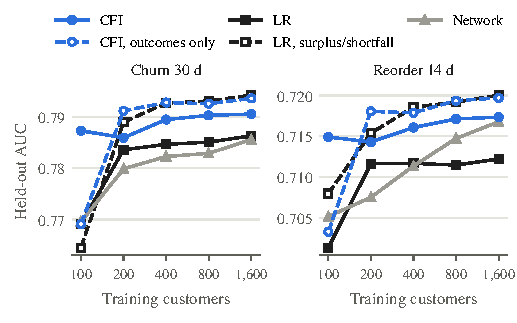
\includegraphics[width=\columnwidth]{fig_small_data.pdf}
\caption{Held-out AUC by the number of training customers, mean of three populations, every model judged on the same 400 held-out customers. CFI, outcomes only: trained on the reorder and churn labels without the survey and behaviour anchors. LR: logistic regression.}\label{fig:small}
\end{figure}

\subsection{Explanations and Drivers}\label{sec:drivers}

Fig.~\ref{fig:example} shows what CFI says about one order, as the dashboard draws it. The order came 6 minutes late, the food was rated half a star below this customer's usual, the fee load was a percentage point of the basket higher, and the app and courier did slightly better than usual. Fit falls from 0.742, for an order exactly as expected, to 0.309, and churn risk rises from 1.0\% to 6.7\%; the food and the lateness carry most of the fall.

\begin{figure}[t]
\centering
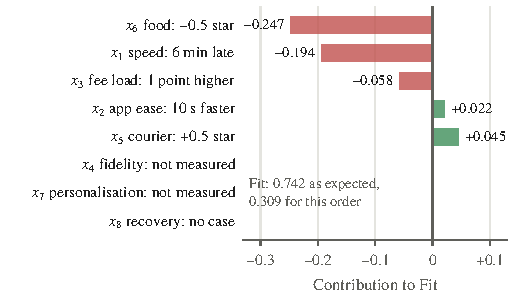
\includegraphics[width=\columnwidth]{fig_example.pdf}
\caption{One order's contributions to Fit (baseline Shapley values against an as-expected order), from the model live on the development service. They add up exactly to the change in Fit.}\label{fig:example}
\end{figure}

Every contribution is exact: in all 670,639 scorings of the driver replays below, the eight contributions to each of the six scores add up to the score's distance from an as-expected order within $10^{-12}$, computed by the same NumPy code the API runs.

An exact explanation is useful only if it points at the right cause. GET /drivers averages each input's contribution to Fit over a restaurant's or courier's orders, subtracts that input's average over all orders (the excess), and ranks groups by their most negative excess. To test it, the simulator planted trouble in 20 populations at each of four sizes, 50 to 400 customers over 90 days (about 660 to 5,130 orders): 80\% of late-delivery incidents went to two of the 40 restaurants, 80\% of cold food to a third, and 80\% of rude-courier incidents to three of the 60 couriers. Every event was replayed through the API's scoring code.

\begin{figure}[t]
\centering
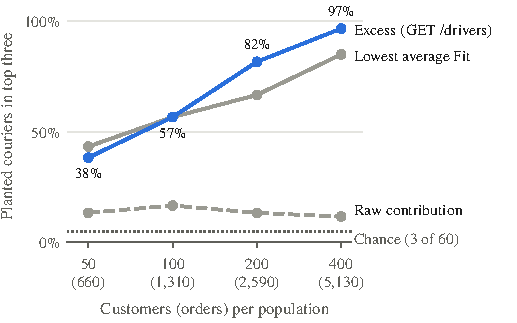
\includegraphics[width=\columnwidth]{fig_drivers.pdf}
\caption{Share of the three worst-ranked couriers that are planted, by population size, under three rankings, mean of 20 populations with its standard error. Naming courier conduct: a hit only if courier conduct is also the courier's first driver.}\label{fig:drivers}
\end{figure}

Restaurants are easy: the three planted kitchens take 98\% of the top three places at 100 customers and all of them from 200, each named for its planted input. Couriers are harder, because rudeness moves only the courier rating, and only on rated orders. From 200 customers the excess earns its place (Fig.~\ref{fig:drivers}): 82\% of its top three couriers are planted at 200 customers and 97\% at 400, against 67\% and 85\% by lowest average Fit and 13\% and 12\% by the raw contribution, since lateness drags every courier alike. Below 200 no ranking finds couriers reliably (38\% to 57\% by the excess). Counting a hit only when the courier is also named for courier conduct changes little (32\% to 97\%).

\subsection{Measurement and the Matrix}\label{sec:matrix}

Measured as v1 events measure, every model loses accuracy: $x_4$ and $x_7$ are never measured, and $x_5$, $x_6$ and $x_8$ only on rated orders and incidents (Table~\ref{tab:prediction}). CFI as deployed, trained with every input measured, scores 0.744 for churn and 0.682 for reorders; retrained without the $x_4$ and $x_7$ paths it scores about the same and is better calibrated (ECE 0.006 against 0.011 for churn). Here the flexible models do better: the unconstrained network leads the deployed CFI by 0.005 for churn and 0.008 for reorders, and logistic regression on surplus and shortfall by 0.004 and 0.006. Which inputs an order measured is itself informative (every order that went wrong is rated), and a model free of CFI's monotone structure can use that; CFI still beats plain logistic regression.

Measurement also blurs the love matrix (Table~\ref{tab:matrix}, from the deployed CFI). With every input measured, each held-out customer's latest quadrant matches the true quadrant 96\% of the time. Measured as events measure, 75\% match, and Lovemarks swell from 56\% to 77\% of customers: an order with no rating and no support case measures nothing that feeds Love, so it scores Love's as-expected value (0.82), above the line. Carrying each input's last measured gap forward is worse still (64\%). The quadrants still sort risk: 30-day churn runs 3.0\% in Lovemark, 9.1\% in Brand, 13.6\% in Fad and 22.7\% in Product. Since states are per order, quadrants move: with every input measured, a customer's quadrant changes between consecutive orders 33\% of the time, close to the simulator's own 32\%, and 15\% as events measure.

\begin{table}[t]
\caption{The Love Matrix Under Three Measurement Rules}\label{tab:matrix}
\centering\footnotesize
\setlength{\tabcolsep}{3.5pt}
\begin{tabular}{@{}l c c c c c@{}}
\toprule
Unmeasured inputs & Agree & Lovemark & Brand & Fad & Product \\
\midrule
All measured & 96 & 56 (2.1) & 15 (6.8) & 16 (13.2) & 13 (20.7) \\
As expected & 75 & 77 (3.0) & 6 (9.1) & 9 (13.6) & 8 (22.7) \\
Carried forward & 64 & 61 (3.1) & 17 (3.6) & 11 (10.0) & 11 (12.0) \\
\bottomrule
\end{tabular}
\par\smallskip\parbox{\columnwidth}{\footnotesize Share of held-out customers in each quadrant by their latest order, \% (30-day churn of the quadrant's orders, \%), and agreement with the true quadrant, \%; CFI as deployed, mean over 20 populations. As expected: what the API does.}
\end{table}

\subsection{Real Orders}\label{sec:olist}

A simulation cannot show that real customers judge gaps the way the theory says. The public Olist dataset \cite{olist2018} can, for speed and fees: 95,824 delivered Brazilian e-commerce orders, each with a promised date and a 1-to-5 review (Fig.~\ref{fig:olist}). An order's gap is the days it arrived before (positive) or after (negative) its promise, as $x_1$ is. A cumulative-logit model of the review \cite{mccullagh1980} on $g_\kappa(\text{gap})$, with $\kappa$ profiled by likelihood on 80\% of customers, gives $\kappa = 7.0$ (95\% likelihood-ratio interval 6.3 to 7.7). On the other fifth, the asymmetric gap explains reviews better than the symmetric one (log-likelihood gain per order over a model with no inputs, 0.048 against 0.032), delivery time alone better than either (0.052), and the two together best (0.060).

\begin{figure}[t]
\centering
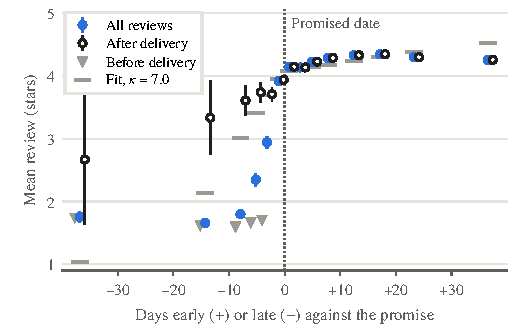
\includegraphics[width=\columnwidth]{fig_olist.pdf}
\caption{Mean Olist review by days early or late against the promise (95\% intervals), for all 95,824 delivered orders (8\% late) and for the reviews written after and before delivery, with the asymmetric fit on all reviews; each point is at its bin's mean gap (bins split at $-20$, $-10$, $-6$, $-4$, $-2$, 0, 2, 4, 6, 10, 15, 20 and 30 days).}\label{fig:olist}
\end{figure}

Much of that gain comes from reviews written before the order arrived. Olist sends its survey when the order arrives or when the promised date passes, whichever is first, and 58\% of late orders were reviewed before delivery, at 1.6 to 1.7 stars for any lateness of two days or more (Fig.~\ref{fig:olist}): a missed promise is itself a gap the customer feels, though not one measured in days. On the 91,170 reviews written after delivery, lateness still costs more than earliness earns: orders up to two days late average 3.9 stars and two to four days late 3.7, against 4.1 up to two days early, and arriving earlier adds nothing (4.1 at two to four days). There $\kappa$ is 12 (8.9 to 15.0), and 3.3 (2.4 to 4.4) within two weeks of the promise: the direction holds, the size depends on the reviews and the range a linear index is fitted to, and the gap explains little (gain 0.003) next to delivery time (0.012). For the fee load (freight over price, against the typical order's), $\kappa$ is 0.15 (0.07 to 0.27, excluding 1): a fee below the usual pleases more than one above it displeases, though it adds almost nothing (gain 0.0002). Olist cannot test the churn head: only 3\% of its customers buy again, and a late first order lowers that only from 3.1\% to 2.8\% ($p = 0.18$, two-proportion test).

\section{System and Dashboard}\label{sec:system}

CFI runs as a working service on Google Cloud. Its development service runs CFI trained on the first population, so the dashboard shows the deployed model of \secref{sec:matrix}.

\begin{figure}[t]
\centering
\resizebox{\columnwidth}{!}{%
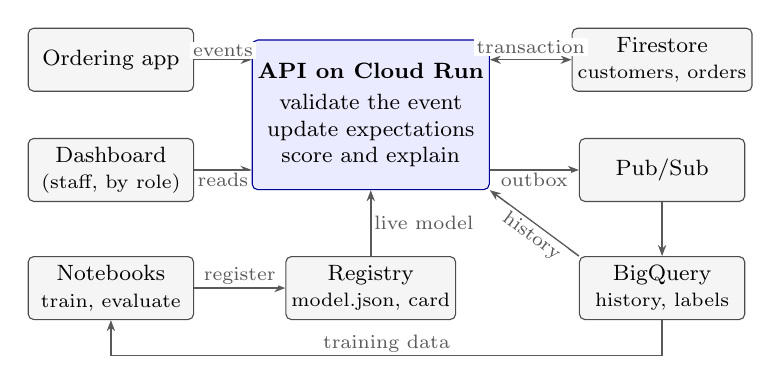
\begin{tikzpicture}[
  >={Stealth[length=4pt]}, font=\footnotesize,
  box/.style={draw=black!70, rounded corners=2pt, fill=black!4, align=center, minimum width=2.1cm, minimum height=0.8cm, inner sep=2pt},
  core/.style={box, fill=blue!8, draw=blue!60!black, minimum width=2.7cm, minimum height=1.9cm},
  flow/.style={->, draw=black!65, line width=0.55pt},
  lab/.style={font=\scriptsize, text=black!65, fill=white, inner sep=1pt}]
\node[core] (api) at (4.2, 2.6) {\textbf{API on Cloud Run}\\[2pt] validate the event\\ update expectations\\ score and explain};
\node[box] (app) at (0.9, 3.3) {Ordering app};
\node[box] (dash) at (0.9, 1.9) {Dashboard\\ \scriptsize(staff, by role)};
\node[box] (fs) at (7.9, 3.3) {Firestore\\ \scriptsize customers, orders};
\node[box] (ps) at (7.9, 1.9) {Pub/Sub};
\node[box] (bq) at (7.9, 0.4) {BigQuery\\ \scriptsize history, labels};
\node[box] (reg) at (4.2, 0.4) {Registry\\ \scriptsize model.json, card};
\node[box] (nb) at (0.9, 0.4) {Notebooks\\ \scriptsize train, evaluate};
\draw[flow] (app) -- node[lab, above] {events} (app -| api.west);
\draw[flow] (dash.east) -- node[lab, below] {reads} (dash -| api.west);
\draw[flow, <->] (fs.west) -- node[lab, above=1pt] {transaction} (fs -| api.east);
\draw[flow] (api.east |- ps) -- node[lab, below] {outbox} (ps.west);
\draw[flow] (ps) -- (bq);
\draw[flow] (bq.north west) -- node[lab, sloped, below, pos=0.45] {history} (api.south east);
\draw[flow] (reg) -- node[lab, right] {live model} (api);
\draw[flow] (nb) -- node[lab, above] {register} (reg);
\draw[flow] (bq.south) -- ++(0,-0.45) -| node[lab, pos=0.25, above] {training data} (nb.south);
\end{tikzpicture}}
\caption{The running system. Every event is scored and explained in one Firestore transaction, then copied through Pub/Sub to BigQuery, where history and labels feed retraining.}\label{fig:system}
\end{figure}

\runin{Pipeline.} The ordering app posts each event to a Flask API on Cloud Run (Fig.~\ref{fig:system}). The API checks it against schema v1 and handles a valid one in a single Firestore transaction: it reads the event's id (a repeat is answered, never applied twice), the customer, the order and the live model; updates the customer's expectations; scores the order and computes its contributions over 256 coalitions; and saves the event, customer, order and a score-history entry together. If another event for the same customer commits first, Firestore runs the transaction again on top of it, so nothing is overwritten. An outbox entry, written in the same transaction, carries every saved document via Pub/Sub to BigQuery; if the API stops between commit and publish, a later request re-sends entries older than a minute, so every document arrives at least once, and BigQuery's views keep one row per event and document. There a scheduled query records every customer's state each day, and the labels are computed as their windows close, ready for retraining.

\runin{Models.} Every trained version's model.json is registered with its SHA-256 hash and a model card that states its data, metrics and limits. Promoting a version, or rolling back, changes one document that every event reads inside its own transaction, so no event is scored by a half-switched model. A golden replay keeps research and service in step: in continuous integration, a fixed log of 795 events goes through the API on the Firestore emulator, and every answer must match the research code's replay of it (fitcore, the package the notebooks and the API share).

\runin{Dashboard.} A React dashboard on Firebase Hosting serves signed-in staff, by role. It shows average Fit, churn risk and the customers at risk, live and by day; the love matrix, with each quadrant's customers now and how they moved since a chosen day; each customer's scores over time, with the contributions behind every order; the drivers of \secref{sec:drivers}, by restaurant or courier over any span of days; and the model registry with each version's card. The matrix does not hide what events cannot measure: customers whose latest order measured nothing that feeds Love sit on a marked band at Love's as-expected value, counted in the legend (122 of 223 simulated customers on the development service; screenshots in the supplement).

\runin{Work, latency and cost.} Each event reads four documents (its id, the customer, the order and the live model), writes five (the four it saves and the outbox entry), later deletes two (the outbox entry, and the event after 30 days), and sends about four rows, 4.4~kB, to BigQuery; at 3.6 events per order, an order leaves about 16~kB of history. On the development service (Cloud Run in Bangkok, 1 vCPU, 512 MiB), 743 events from 50 new simulated customers, sent one at a time from a laptop in Bangkok, took 1.1~ms each at the median in one process, scoring included; 175~ms inside Cloud Run, by its request log (95th percentile 208~ms); and 416~ms door to door through Firebase Hosting (592~ms). The rest is storage and messaging round trips, not timed apart, and one client at a time says nothing about contention under load. At the list rates of Google Cloud's cheapest regions beyond the free tier, 1,000 events cost about \$0.011 (\$0.006 of Firestore operations, \$0.005 of Cloud Run time, under \$0.001 of Pub/Sub and BigQuery); the development service's region costs more, Firestore up to twice as much.

\section{Discussion and Limitations}\label{sec:discussion}

\runin{What simulation can show.} The simulator shares CFI's connections and signs, so the study shows what the constraints cost and whether training finds states that are there, not that real customers have them. \secref{sec:robust} breaks one assumption at a time, in three populations; worlds with another grouping of inputs, saturating effects or states carried between orders are the next test. Real data has tested two inputs, on Olist: lateness is asymmetric, by an amount that depends on the reviews used, and fees run the other way ($\kappa = 0.15$), which CFI's $\kappa > 1$ cannot represent, so each input's $\kappa$ should be estimated, with room below 1, on real orders. Gaps also adapt, and on Olist the level, delivery time, explains reviews better than the gap, so a level input belongs beside the gaps.

\runin{Measurement.} CFI is only as good as what events measure. Two inputs, order fidelity and personalisation, are not in v1 events, and ratings arrive on a minority of orders. Scoring an unmeasured input as expected crowds customers into the Lovemark quadrant, and flexible models then predict better than CFI (\secref{sec:matrix}). We keep the quadrant lines at 0.5; what should change is what is measured and shown: item-level accuracy and recommendation outcomes in the events, which inputs were measured as an input of its own, and scores marked by how many inputs were measured.

\runin{States and anchors.} CFI's states are per order; a customer carries memory only through the expectations, so a quadrant can change with any order, as it does a third of the time in simulation. The theory's relationships accumulate, and a state carried between orders would match them better. In real data two anchors would reuse inputs (the average rating draws on $x_5$ and $x_6$, checkout time is $x_2$'s raw measure; the simulator draws behaviours from the true states), so a deployment should anchor states with behaviours not computed from their own inputs.

\runin{Explanation is not causation.} Contributions are exact for the model, not causal for the customer: a driver says which gap moved this customer's Fit in CFI, not that fixing it will win the customer back. That needs controlled experiments before any action is automated, and the driver test still lacks a simple baseline such as each courier's mean rating.

\runin{Privacy.} CFI keeps per-customer states derived from behaviour. The service uses no personal attributes, keeps raw events for 30 days, and restricts the dashboard to staff by role; a deployment still needs consent, retention and access rules, and checks that a low Fit never lowers the service a customer receives.

\runin{Code and data.} The code, the result files and a supplement with every setting and further tables are public:\\{\footnotesize\url{https://github.com/ruinogenesis/customer-fit-intelligence}}.

\section{Conclusion and Future Work}\label{sec:conclusion}

When the theory is right, fixing a network's structure from it cost CFI little in prediction: within 0.004 AUC of the best comparator on the same inputs, and within 0.003 of the true Fit with history. In return its hidden units are named states with fixed signs that follow the truth beyond what the structure alone gives, every score is explained exactly, its anchors let it learn from 100 customers, and its drivers find planted problems once groups have enough orders. Two results temper this: with only what events measure today, flexible models predict better, and on real orders lateness is asymmetric by an amount that depends on the reviews, while fees run the other way. Next, CFI will be trained on its first months of real orders, with $\kappa$ per input allowed below 1, states carried between orders and inputs for what events do not yet measure; driver-led actions will be tested in controlled experiments before any is automated.

\footnotesize
\begin{thebibliography}{19}
\setlength{\itemsep}{1pt}
\bibitem{neslin2006} S.~A. Neslin, S.~Gupta, W.~Kamakura, J.~Lu, and C.~H. Mason, ``Defection detection: Measuring and understanding the predictive accuracy of customer churn models,'' \textit{J. Marketing Res.}, vol.~43, no.~2, pp.~204--211, 2006.
\bibitem{fader2005} P.~S. Fader, B.~G.~S. Hardie, and K.~L. Lee, ```Counting your customers' the easy way: An alternative to the Pareto/NBD model,'' \textit{Marketing Sci.}, vol.~24, no.~2, pp.~275--284, 2005.
\bibitem{oliver1980} R.~L. Oliver, ``A cognitive model of the antecedents and consequences of satisfaction decisions,'' \textit{J. Marketing Res.}, vol.~17, no.~4, pp.~460--469, 1980.
\bibitem{mittal1998} V.~Mittal, W.~T. Ross, Jr., and P.~M. Baldasare, ``The asymmetric impact of negative and positive attribute-level performance on overall satisfaction and repurchase intentions,'' \textit{J. Marketing}, vol.~62, no.~1, pp.~33--47, 1998.
\bibitem{roberts2004} K.~Roberts, \textit{Lovemarks: The Future Beyond Brands}. New York, NY, USA: powerHouse Books, 2004.
\bibitem{reichheld2003} F.~F. Reichheld, ``The one number you need to grow,'' \textit{Harvard Bus. Rev.}, vol.~81, no.~12, pp.~46--54, 2003.
\bibitem{morris2019} T.~P. Morris, I.~R. White, and M.~J. Crowther, ``Using simulation studies to evaluate statistical methods,'' \textit{Statist. Med.}, vol.~38, no.~11, pp.~2074--2102, 2019.
\bibitem{olist2018} Olist, ``Brazilian e-commerce public dataset by Olist,'' Kaggle, 2018. Accessed: Nov. 19, 2026. [Online]. Available: \url{https://www.kaggle.com/datasets/olistbr/brazilian-ecommerce}
\bibitem{lundberg2017} S.~M. Lundberg and S.-I. Lee, ``A unified approach to interpreting model predictions,'' in \textit{Proc. Adv. Neural Inf. Process. Syst. 30}, 2017, pp.~4765--4774.
\bibitem{sundararajan2020} M.~Sundararajan and A.~Najmi, ``The many Shapley values for model explanation,'' in \textit{Proc. 37th Int. Conf. Mach. Learn.}, PMLR vol.~119, 2020, pp.~9269--9278.
\bibitem{morgan1994} R.~M. Morgan and S.~D. Hunt, ``The commitment-trust theory of relationship marketing,'' \textit{J. Marketing}, vol.~58, no.~3, pp.~20--38, 1994.
\bibitem{berry2002} L.~L. Berry, K.~Seiders, and D.~Grewal, ``Understanding service convenience,'' \textit{J. Marketing}, vol.~66, no.~3, pp.~1--17, 2002.
\bibitem{friedman2001} J.~H. Friedman, ``Greedy function approximation: A gradient boosting machine,'' \textit{Ann. Statist.}, vol.~29, no.~5, pp.~1189--1232, 2001.
\bibitem{rudin2019} C.~Rudin, ``Stop explaining black box machine learning models for high stakes decisions and use interpretable models instead,'' \textit{Nature Mach. Intell.}, vol.~1, no.~5, pp.~206--215, 2019.
\bibitem{karpatne2017} A.~Karpatne \textit{et al.}, ``Theory-guided data science: A new paradigm for scientific discovery from data,'' \textit{IEEE Trans. Knowl. Data Eng.}, vol.~29, no.~10, pp.~2318--2331, 2017.
\bibitem{koh2020} P.~W. Koh \textit{et al.}, ``Concept bottleneck models,'' in \textit{Proc. 37th Int. Conf. Mach. Learn.}, PMLR vol.~119, 2020, pp.~5338--5348.
\bibitem{you2017} S.~You, D.~Ding, K.~Canini, J.~Pfeifer, and M.~Gupta, ``Deep lattice networks and partial monotonic functions,'' in \textit{Proc. Adv. Neural Inf. Process. Syst. 30}, 2017, pp.~2981--2989.
\bibitem{fornell1996} C.~Fornell, M.~D. Johnson, E.~W. Anderson, J.~Cha, and B.~E. Bryant, ``The American customer satisfaction index: Nature, purpose, and findings,'' \textit{J. Marketing}, vol.~60, no.~4, pp.~7--18, 1996.
\bibitem{mccullagh1980} P.~McCullagh, ``Regression models for ordinal data,'' \textit{J. Roy. Statist. Soc. B}, vol.~42, no.~2, pp.~109--142, 1980.
\end{thebibliography}

\end{document}
